
\hl{[[Here I tried to give an overview about different subsections of the background section]]}

In this section, we provide some background that explains our methodology for data collection and data analysis towards debugging and locating potential root causes of the unexpected behavior. 
%

\hl{Section} \ref{subsec:parlot} \hl{:}
The main source of whole-program dynamic behavior is provided by ParLOT, a dynamic binary tracing tool that captures all function calls and returns and compresses them on the fly (section \ref{subsec:parlot}), producing a set of highly compact \textit{ParLOT Traces} (PTs).
\\
%
\hl{Section} \ref{subsec:nlr} \hl{:}
After pre-processing, a loop-detection-based lossless data reduction mechanism is applied to each PT to simplify the collected data and to reflect facts about loop structures (section \ref{subsec:nlr}).
%
\\
\hl{Section} \ref{subsec:fca} \hl{:}
Whole-program analysis in HPC applications only makes sense when the analysis of each thread's control flow is performed across all threads and processes.
%
Inspired by other work \cite{weberStructural} \cite{Alqadah2011} \cite{Ignatov17} \cite{latticeForDistConst}, we have used FCA \cite{clbook} to integrate the collected data into a single data structure, from which we extract valuable information about different aspects of the execution (section \ref{subsec:fca}).
%
The major advantage of FCA is that we can extract a full pair-wise similarity score matrix for all traces of a single execution in an efficient and scalable way based on attributes that we extract from the pre-processed traces.
%
Relying on similarities of traces, we classify PTs into equivalent-behavior classes.
%
This way, we reduce the search space from thousands of long PTs to just a few classes of simplified traces without losing important information.
\\
\hl{Section} \ref{subsec:ranking} \hl{:}
Given the wide ar


Section \ref{subsec:ranking} \hl{ talk about how we rank PTs based on their comparison with corresponding PTs from bug-free execution and how we pick some PTs for deeper study.}
\\
Section \ref{subsec:diffnlr}\hl{ explain why visualizing diffs of a pair of PT is useful and some background about it.}




% Binary tracing
\subsection{ParLOT: Efficient Trace Collection}
\label{subsec:parlot}

The executable of HPC applications is often a combination of a large code base and a complex build system with numerous dependencies and libraries. Injecting instrumentation code to the source code, as in \hl{traditional tools like [????]}, is difficult in the HPC space. Also, recompilation of the application with compiler wrappers, as in TAU \cite{tau} and Score-p \cite{scorep}, may break the build system.
The instrumentation and tracing mechanism of existing tools are often dependent on other libraries that are need to be present on the target system for trace collection. \hl{Example: STAT} \cite{stat} and \hl{AutomaDeD} \cite{automaded-laguna} that requires \hl{Dyninst} \cite{dyninst} for instrumentation and \hl{MRNet} \cite{mrnet} and \hl{ TBON} \cite{tbon}.
%
To enable comprehensive data collection in combination with low time and space overhead, HPC program analysis tools often sacrifice one for the other. However, ParLOT collects whole-program function call traces at as low as library level, while incrementally compressing traces on-the-fly and leaving the majority of the system bandwidth for the application.
%
ParLOT collects \textit{whole} program function call traces with the mindset of \textit{paying a little upfront and saving resource and time cost of reproducing the bug later}.
%
ParLOT instruments the entry and exit point of each function in the binary using Pin \cite{pin} (fig.~\ref{fig.parlotOverview}). Each ParLOT Trace contains full sequence of function calls and returns for every thread of the application code, reflecting the dynamic control flow and call stack.
%
Here we define ParLOT Trace, as we refer to it in the paper:

\begin{definition}{ParLOT Trace (PT)}
A ParLOT Trace $(PT)$ is a sequence of ordered integers $<f_i,...,f_j>$ where $f_0$ represents a \textit{return} and $f_k$ is the ID of \textit{function k} ($k \neq 0$).
\end{definition}
%
Note that the $PT$ is the pre-processed (decompressed and filtered) version of the ParLOT traces. The native format of ParLOT traces is highly compressed using a custom algorithm.
%
Note that $PT_{p.t}$ refers to the $PT$ that belongs to process $p$ and thread $t$ of that process.
%
\begin{figure}[t]
\caption{ParLOT Overview}
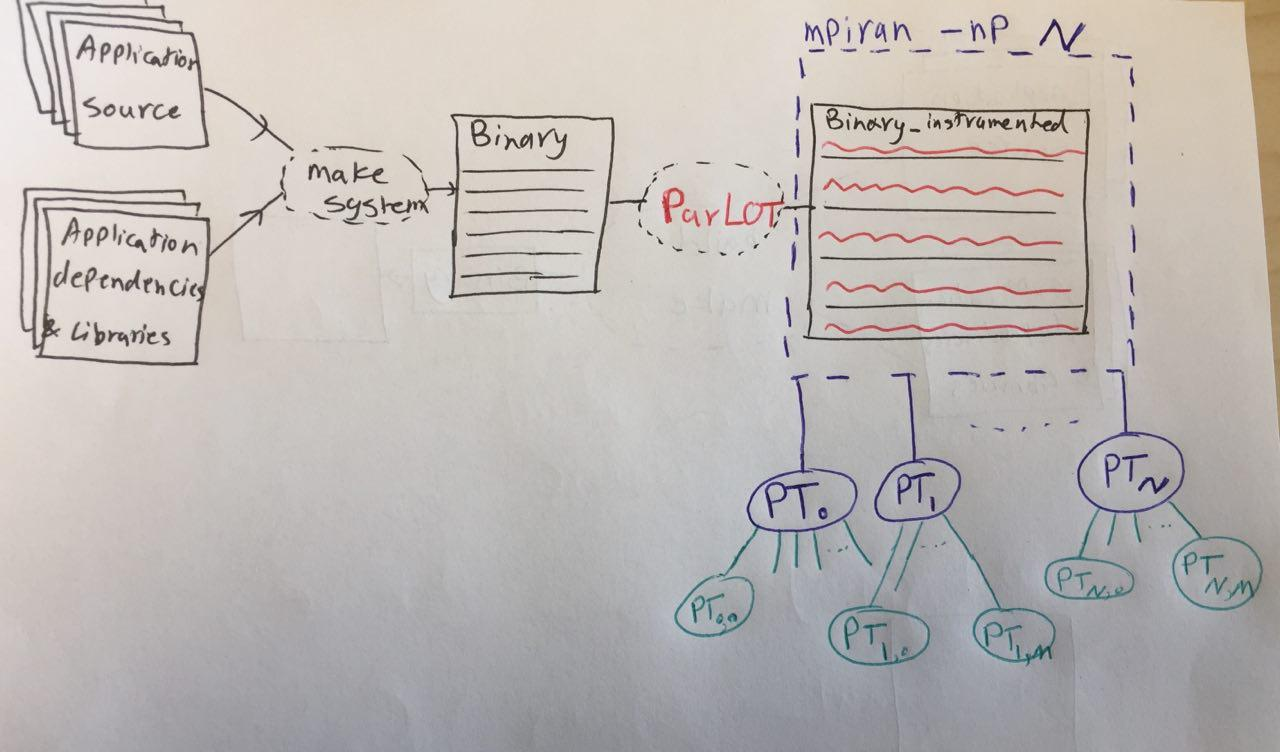
\includegraphics[width=0.45\textwidth]{figs/parlotOverview.jpg}
\label{fig.parlotOverview}
\end{figure}

\hl{What else do we need here?}

% NLRs
\subsection{Loop structure detection}
\label{subsec:nlr}

HPC applications and resources are of great interest to scientists and engineers for simulating \textit{iterative} kernels. Computer simulation of fluid dynamics, partial differential equations, the Gauss-Seidel method, and finite element methods in form of stencil codes, all include a main outer loop that iterates over some elements (i.e., timesteps) and updates the elements.
%
This character of typical HPC applications makes PTs very long (often millions or billions of entries) with a relatively small number (hundreds to thousands) of distinct elements (i.e., function IDs).
%
We propose a representation of PT elements (intra-PT compression) in form of \textit{loop structures}, such that PT = sequence of repetitive patterns (i.e., loops). In other words, each PT is a sequence of \textit{Loop Bodies (LB)} that repeated \textit{Loop Count (LC)} times, consecutively.
%


\subsubsection{Loops definition}

According to Makoto Kobayashi's \cite{kobayashi-84} definition of loops, an occurrence of a \textit{loop} is defined as \textit{a sequence of elements} in which a particular sequence of \textit{distinct elements} (called the \textit{cycle} of the loop) is successively repeated.
%
Later, Alain Ketterlin \cite{Ketterlin-nlr} expanded this definition to numerical values for compressing and predicting memory access addresses and designed the Nested Loop Recognition (NLR) algorithm.
%
The basic idea behind the NLR algorithm is that a linear function model can be extracted from the linear progression in a sequence of numbers, and these linear functions form a tree in which the depth of each node is the depth of a \textit{nested} loop (the outermost loop's function is the root of the tree with depth 0).
%
We have modified the NLR algorithm to make it suitable for PTs.
%
Each repetitive pattern and its frequency of consecutive appearances would be compressed to a single \textit{Loop Structure (LS)} entry.
%
\begin{definition}{Loop Structure} $LS = LB \; \hat{} \; LC$ where $LB  = <pt_i,...,pt_j>$ ($0 <= i < j < len(PT)$) that occur $LC$ times is in a sub-sequence $<pt_i,...,pt_k>$ ($k = 3j, k < len(PT)$)

\end{definition}
%
By converting each PT into a sequence of $LS_i$, we reduce the length of PT by a factor of $\sum_i len(LB_i) * LC_i$.
%
Later we will explain how this lossless representation of PTs eases the process of diffing between a pair of PTs.

\hl{What else do we need here?}

% CLs
\subsection{Equivalencing behavior via FCA}
\label{subsec:fca}
Reducing the search space from thousands of PTs to just a few groups of equivalent PTs (i.e., inter-PT compression) not only requires a similarity measure based on a call matrix but also a scheme that is efficient even for large process counts.
%
Since a pair-wise comparison of all processes is highly inefficient, we use \textit{concept lattices} that stem from \textit{formal concept analysis}(FCA) \cite{clbook} to store and compute groups of similar PTs.
%
A concept lattice is based on a \textit{formal context} \cite{clbook}, which is a triple $(O, A, I)$, where $O$ is a set of \textbf{objects}, $A$ a set of \textbf{attributes}, and $I \subseteq O \times A$ an incidence relation. The incidence relation associates each object with a set of attributes.
%
Due to its valuable properties, especially its \textit{partial order}, FCA has been used widely in computer science fields from machine learning and data mining \cite{Ignatov17} to distributed systems \cite{latticeForDistConst}.
%
However, since we are only interested in grouping similar PTs in this work, we only take advantage of similarity measures \cite{Alqadah2011} of concept lattices and leave other properties for future work.
%
Due to typical HPC application topologies such as SPMD, master/worker and odd/even where multiple processes/threads behave similarly, our experiments show that large numbers of PTs can be reduced to just a few groups.
%

\begin{frame}{}
  \lstset{language=C}
 \begin{lstlisting}
main(){
 int rank;
 int src;
 MPI_Init()
 MPI_Comm_size(MPI_COMM_WORLD)
 MPI_Comm_rank(MPI_COMM_WORLD,&rank)
 if (rank != 0) {
  MPI_Send(0) // Send to rank 0
 } else{ /* rank = 0
  MPI_Recv(1) // Receive from rank 1
  MPI_Recv(2) // Receive from rank 2
  MPI_Recv(3) // Receive from rank 3
 }
 MPI_Finalize()
}
\end{lstlisting}
\end{frame}



\begin{table}[]
\caption{Formal Context of odd/even sort example}
\label{tab:sampleContext}
\scalebox{0.7}{
\begin{tabular}{l|cccccc}
 & \multicolumn{1}{l}{MPI\_Init()} & \multicolumn{1}{l}{MPI\_Comm\_Size()} & \multicolumn{1}{l}{MPI\_Comm\_Rank()} & \multicolumn{1}{l}{L0} & \multicolumn{1}{l}{L1} & \multicolumn{1}{l}{MPI\_Finalize()} \\ \hline
Trace 0 & $\times$ & $\times$ & $\times$ & $\times$ &  & $\times$ \\
Trace 1 & $\times$ & $\times$ & $\times$ &  & $\times$ & $\times$ \\
Trace 2 & $\times$ & $\times$ & $\times$ & $\times$ &  & $\times$ \\
Trace 3 & $\times$ & $\times$ & $\times$ &  & $\times$ & $\times$
\end{tabular}}
\end{table}

\begin{figure}[t]
\centering
\scalebox{0.5}{
\includegraphics[width=3.4in]{figs/{sample}.pdf}}
\caption{Sample Concept Lattice from Obj-Atr Context in table\ref{tab:sampleContext}}

\label{fig:sampleCL}
\end{figure}

\begin{figure}[t]
\centering
\scalebox{0.5}{
\includegraphics[width=3.4in]{figs/{sample-reduced}.pdf}}
\caption{Concept Lattice with reduced labels}
\label{fig:sampleCL}
\end{figure}





\subsubsection{Jaccard Similarity Scores}

\hl{- Some background about Jaccard Similarity Score

- How to obtain full pair-wise Jaccard Similarity Matrix (JSM) from a concept lattice (e.g., LCA approach)
}
\begin{figure}[t]
\centering
\scalebox{0.8}{
\includegraphics[width=3.4in]{figs/{fancy1}.pdf}}
\caption{Pair-wise Jaccard Similarity Matrix (JSM) of MPI processes in Sample code}
\label{fig:jsm}
\end{figure}


\hl{More explanations about concept lattices, CL construction appears in DiffTrace Components section. What else do we need here?}


\subsection{Ranking Suspicious PTs}
\label{subsec:ranking}

\hl{Explanations about how we rank PTs based on their significant difference with respect to bug-free version}


\subsection{diffNLR: Reflecting differences}
\label{subsec:diffnlr}
\hl{From fig we can see that PT0 and PT1 are in different groups with similarity of XX.}
%
\\
Inspired by \texttt{diff} original algorithm\cite{diff-myers} that has bin used in Git and GNU Diff, we visualize the differences of a pair of PT as shown in fig \ref{fig:sampleDiffNLR}.
\\
This visualization reflects of the differences of \textbf{occurrences} of PT elements and their \textbf{orders}.
\\
In section \ref{sec:experimental} we show how this visualization can help us locating the points of divergence in PTs, and potential bug manifestation and root cause.

\begin{figure}[t]
\centering
\scalebox{0.5}{
\includegraphics[width=3.4in]{figs/{sampleDiffNLR}.png}}
\caption{Sample diffNLR}
\label{fig:sampleDiffNLR}
\end{figure}


